\section{Ui file for menu and action
entries}\label{ui-file-for-menu-and-action-entries}

\subsection{Ui file for menu}\label{ui-file-for-menu}

You may have thought that building menus was really bothersome. Yes, the
program was complicated and it needs lots of time to code them. The
situation is similar to building widgets. When we built widgets, using
ui file was a good way to avoid such complication. The same goes for
menus.

The ui file for menus has interface and menu tags. The file starts and
ends with interface tags.

\begin{lstlisting}[language=XML]
<interface>
  <menu id="menubar">
  </menu>
</interface>
\end{lstlisting}

\passthrough{\lstinline!menu!} tag corresponds to GMenu object.
\passthrough{\lstinline!id!} attribute defines the name of the object.
It will be referred by GtkBuilder.

\begin{lstlisting}[language=XML]
<submenu>
  <attribute name="label">File</attribute>
    <item>
      <attribute name="label">New</attribute>
      <attribute name="action">win.new</attribute>
    </item>
</submenu>
\end{lstlisting}

\passthrough{\lstinline!item!} tag corresponds to an item in the GMenu
which has the same structure as GMenuItem. The item above has a label
attribute. Its value is ``New''. The item also has an action attribute
and its value is ``win.new''. ``win'' is a prefix and ``new'' is an
action name. \passthrough{\lstinline!submenu!} tag corresponds to both
GMenuItem and GMenu. The GMenuItem has a link to GMenu.

The ui file above can be described as follows.

\begin{lstlisting}[language=XML]
<item>
  <attribute name="label">File</attribute>
    <link name="submenu">
      <item>
        <attribute name="label">New</attribute>
        <attribute name="action">win.new</attribute>
      </item>
    </link>
</item>
\end{lstlisting}

\passthrough{\lstinline!link!} tag expresses the link to submenu. And at
the same time it also expresses the submenu itself. This file
illustrates the relationship between the menus and items better than the
prior ui file. But \passthrough{\lstinline!submenu!} tag is simple and
easy to understand. So, we usually prefer the former ui style.

For further information, see
\href{https://docs.gtk.org/gtk4/class.PopoverMenu.html\#menu-models}{GTK
4 API reference -- PopoverMenu}.

The following is a screenshot of the sample program
\passthrough{\lstinline!menu3!}. It is located in the directory
src/menu3.

\begin{figure}
\centering
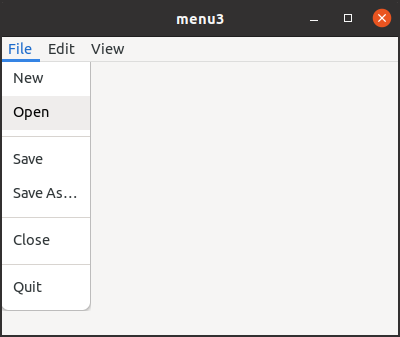
\includegraphics[width=6cm,height=5.055cm]{../image/menu3.png}
\caption{menu3}
\end{figure}

The following is the ui file for \passthrough{\lstinline!menu3!}.

\begin{lstlisting}[language=XML, numbers=left]
<?xml version="1.0" encoding="UTF-8"?>
<interface>
  <menu id="menubar">
    <submenu>
      <attribute name="label">File</attribute>
      <section>
        <item>
          <attribute name="label">New</attribute>
          <attribute name="action">app.new</attribute>
        </item>
        <item>
          <attribute name="label">Open</attribute>
          <attribute name="action">app.open</attribute>
        </item>
      </section>
      <section>
        <item>
          <attribute name="label">Save</attribute>
          <attribute name="action">win.save</attribute>
        </item>
        <item>
          <attribute name="label">Save As…</attribute>
          <attribute name="action">win.saveas</attribute>
        </item>
      </section>
      <section>
        <item>
          <attribute name="label">Close</attribute>
          <attribute name="action">win.close</attribute>
        </item>
      </section>
      <section>
        <item>
          <attribute name="label">Quit</attribute>
          <attribute name="action">app.quit</attribute>
        </item>
      </section>
    </submenu>
    <submenu>
      <attribute name="label">Edit</attribute>
      <section>
        <item>
          <attribute name="label">Cut</attribute>
          <attribute name="action">app.cut</attribute>
        </item>
        <item>
          <attribute name="label">Copy</attribute>
          <attribute name="action">app.copy</attribute>
        </item>
        <item>
          <attribute name="label">Paste</attribute>
          <attribute name="action">app.paste</attribute>
        </item>
      </section>
      <section>
        <item>
          <attribute name="label">Select All</attribute>
          <attribute name="action">app.selectall</attribute>
        </item>
      </section>
    </submenu>
    <submenu>
      <attribute name="label">View</attribute>
      <section>
        <item>
          <attribute name="label">Full Screen</attribute>
          <attribute name="action">win.fullscreen</attribute>
        </item>
      </section>
    </submenu>
  </menu>
</interface>
\end{lstlisting}

The ui file is converted to the resource by the resource compiler
\passthrough{\lstinline!glib-compile-resouces!} with xml file.

\begin{lstlisting}[language=XML, numbers=left]
<?xml version="1.0" encoding="UTF-8"?>
<gresources>
  <gresource prefix="/com/github/ToshioCP/menu3">
    <file>menu3.ui</file>
  </gresource>
</gresources>
\end{lstlisting}

GtkBuilder builds menus from the resource.

\begin{lstlisting}[language=C]
GtkBuilder *builder = gtk_builder_new_from_resource ("/com/github/ToshioCP/menu3/menu3.ui");
GMenuModel *menubar = G_MENU_MODEL (gtk_builder_get_object (builder, "menubar"));

gtk_application_set_menubar (GTK_APPLICATION (app), menubar);
g_object_unref (builder);
\end{lstlisting}

The builder instance is freed after the GMenuModel
\passthrough{\lstinline!menubar!} is inserted to the application. If you
do it before the insertion, bad thing will happen -- your computer might
freeze. It is because you don't own the
\passthrough{\lstinline!menubar!} instance. The function
\passthrough{\lstinline!gtk\_builder\_get\_object!} just returns the
pointer to \passthrough{\lstinline!menubar!} and doesn't increase the
reference count of \passthrough{\lstinline!menubar!}. So, if you
released \passthrough{\lstinline!bulder!} before
\passthrough{\lstinline!gtk\_application\_set\_menubar!},
\passthrough{\lstinline!builder!} would be destroyed and
\passthrough{\lstinline!menubar!} as well.

\subsection{Action entry}\label{action-entry}

The coding for building actions and signal handlers is bothersome work
as well. Therefore, it should be automated. You can implement them
easily with GActionEntry structure and
\passthrough{\lstinline!g\_action\_map\_add\_action\_entries!} function.

GActionEntry contains action name, signal handlers, parameter and state.

\begin{lstlisting}[language=C]
typedef struct _GActionEntry GActionEntry;

struct _GActionEntry
{
  /* action name */
  const char *name;
  /* activate handler */
  void (* activate) (GSimpleAction *action, GVariant *parameter, gpointer user_data);
  /* the type of the parameter given as a single GVariant type string */
  const char *parameter_type;
  /* initial state given in GVariant text format */
  const char *state;
  /* change-state handler */
  void (* change_state) (GSimpleAction *action, GVariant *value, gpointer user_data);
  /*< private >*/
  gsize padding[3];
};
\end{lstlisting}

For example, the actions in the previous section are:

\begin{lstlisting}[language=C]
{ "fullscreen", NULL, NULL, "false", fullscreen_changed }
{ "color", color_activated, "s", "'red'", NULL }
{ "quit", quit_activated, NULL, NULL, NULL },
\end{lstlisting}

\begin{itemize}
\tightlist
\item
  Fullscreen action is stateful, but doesn't have parameters. So, the
  third element (parameter type) is NULL.
  \href{https://docs.gtk.org/glib/gvariant-text.html}{GVariant text
  format} provides ``true'' and ``false'' as boolean GVariant values.
  The initial state of the action is false (the fourth element). It
  doesn't have activate handler, so the second element is NULL. Instead,
  it has change-state handler. The fifth element
  \passthrough{\lstinline!fullscreen\_changed!} is the handler.
\item
  Color action is stateful and has a parameter. The parameter type is
  string.
  \href{https://docs.gtk.org/glib/gvariant-format-strings.html}{GVariant
  format strings} provides string formats to represent GVariant types.
  The third element ``s'' means GVariant string type. GVariant text
  format defines that strings are surrounded by single or double quotes.
  So, the string red is `red' or ``red''. The fourth element is
  \passthrough{\lstinline!"'red'"!}, which is a C string format and the
  string is `red'. You can write \passthrough{\lstinline!"\\"red\\""!}
  instead. The second element \passthrough{\lstinline!color\_activated!}
  is the activate handler. The action doesn't have change-state handler,
  so the fifth element is NULL.
\item
  Quit action is non-stateful and has no parameter. So, the third and
  fourth elements are NULL. The second element
  \passthrough{\lstinline!quit\_activated!} is the activate handler. The
  action doesn't have change-state handler, so the fifth element is
  NULL.
\end{itemize}

The function
\passthrough{\lstinline!g\_action\_map\_add\_action\_entries!} does
everything to create GSimpleAction instances and add them to a
GActionMap (an application or window).

\begin{lstlisting}[language=C]
const GActionEntry app_entries[] = {
  { "color", color_activated, "s", "'red'", NULL },
  { "quit", quit_activated, NULL, NULL, NULL }
};
g_action_map_add_action_entries (G_ACTION_MAP (app), app_entries,
                                 G_N_ELEMENTS (app_entries), app);
\end{lstlisting}

The code above does:

\begin{itemize}
\tightlist
\item
  Builds the ``color'' and ``quit'' actions
\item
  Connects the action and the ``activate'' signal handlers
  (\passthrough{\lstinline!color\_activated!} and
  \passthrough{\lstinline!quit\_activated!}).
\item
  Adds the actions to the action map \passthrough{\lstinline!app!}.
\end{itemize}

The same goes for the other action.

\begin{lstlisting}[language=C]
const GActionEntry win_entries[] = {
  { "fullscreen", NULL, NULL, "false", fullscreen_changed }
};
g_action_map_add_action_entries (G_ACTION_MAP (win), win_entries,
                                 G_N_ELEMENTS (win_entries), win);
\end{lstlisting}

The code above does:

\begin{itemize}
\tightlist
\item
  Builds the ``fullscreen'' action.
\item
  Connects the action and the signal handler
  \passthrough{\lstinline!fullscreen\_changed!}
\item
  Its initial state is set to false.
\item
  Adds the action to the action map \passthrough{\lstinline!win!}.
\end{itemize}

\subsection{Example}\label{example}

Source files are \passthrough{\lstinline!menu3.c!},
\passthrough{\lstinline!menu3.ui!},
\passthrough{\lstinline!menu3.gresource.xml!} and
\passthrough{\lstinline!meson.build!}. They are in the directory
src/menu3. The following are \passthrough{\lstinline!menu3.c!} and
\passthrough{\lstinline!meson.build!}.

\begin{lstlisting}[language=C, numbers=left]
#include <gtk/gtk.h>

static void
new_activated (GSimpleAction *action, GVariant *parameter, gpointer user_data) {
}

static void
open_activated (GSimpleAction *action, GVariant *parameter, gpointer user_data) {
}

static void
save_activated (GSimpleAction *action, GVariant *parameter, gpointer user_data) {
}

static void
saveas_activated (GSimpleAction *action, GVariant *parameter, gpointer user_data) {
}

static void
close_activated (GSimpleAction *action, GVariant *parameter, gpointer user_data) {
  GtkWindow *win = GTK_WINDOW (user_data);

  gtk_window_destroy (win);
}

static void
cut_activated (GSimpleAction *action, GVariant *parameter, gpointer user_data) {
}

static void
copy_activated (GSimpleAction *action, GVariant *parameter, gpointer user_data) {
}

static void
paste_activated (GSimpleAction *action, GVariant *parameter, gpointer user_data) {
}

static void
selectall_activated (GSimpleAction *action, GVariant *parameter, gpointer user_data) {
}

static void
fullscreen_changed (GSimpleAction *action, GVariant *state, gpointer user_data) {
  GtkWindow *win = GTK_WINDOW (user_data);

  if (g_variant_get_boolean (state))
    gtk_window_maximize (win);
  else
    gtk_window_unmaximize (win);
  g_simple_action_set_state (action, state);
}

static void
quit_activated (GSimpleAction *action, GVariant *parameter, gpointer user_data) {
  GApplication *app = G_APPLICATION (user_data);

  g_application_quit (app);
}

static void
app_activate (GApplication *app) {
  GtkWidget *win = gtk_application_window_new (GTK_APPLICATION (app));

  const GActionEntry win_entries[] = {
    { "save", save_activated, NULL, NULL, NULL },
    { "saveas", saveas_activated, NULL, NULL, NULL },
    { "close", close_activated, NULL, NULL, NULL },
    { "fullscreen", NULL, NULL, "false", fullscreen_changed }
  };
  g_action_map_add_action_entries (G_ACTION_MAP (win), win_entries, G_N_ELEMENTS (win_entries), win);

  gtk_application_window_set_show_menubar (GTK_APPLICATION_WINDOW (win), TRUE);

  gtk_window_set_title (GTK_WINDOW (win), "menu3");
  gtk_window_set_default_size (GTK_WINDOW (win), 400, 300);
  gtk_window_present (GTK_WINDOW (win));
}

static void
app_startup (GApplication *app) {
  GtkBuilder *builder = gtk_builder_new_from_resource ("/com/github/ToshioCP/menu3/menu3.ui");
  GMenuModel *menubar = G_MENU_MODEL (gtk_builder_get_object (builder, "menubar"));

  gtk_application_set_menubar (GTK_APPLICATION (app), menubar);
  g_object_unref (builder);

  const GActionEntry app_entries[] = {
    { "new", new_activated, NULL, NULL, NULL },
    { "open", open_activated, NULL, NULL, NULL },
    { "cut", cut_activated, NULL, NULL, NULL },
    { "copy", copy_activated, NULL, NULL, NULL },
    { "paste", paste_activated, NULL, NULL, NULL },
    { "selectall", selectall_activated, NULL, NULL, NULL },
    { "quit", quit_activated, NULL, NULL, NULL }
  };
  g_action_map_add_action_entries (G_ACTION_MAP (app), app_entries, G_N_ELEMENTS (app_entries), app);
}

#define APPLICATION_ID "com.github.ToshioCP.menu3"

int
main (int argc, char **argv) {
  GtkApplication *app;
  int stat;

  app = gtk_application_new (APPLICATION_ID, G_APPLICATION_DEFAULT_FLAGS);
  g_signal_connect (app, "startup", G_CALLBACK (app_startup), NULL);
  g_signal_connect (app, "activate", G_CALLBACK (app_activate), NULL);

  stat =g_application_run (G_APPLICATION (app), argc, argv);
  g_object_unref (app);
  return stat;
}
\end{lstlisting}

meson.build

\begin{lstlisting}[numbers=left]
project('menu3', 'c')

gtkdep = dependency('gtk4')

gnome=import('gnome')
resources = gnome.compile_resources('resources','menu3.gresource.xml')

sourcefiles=files('menu3.c')

executable('menu3', sourcefiles, resources, dependencies: gtkdep)
\end{lstlisting}

Action handlers need to follow the following format.

\begin{lstlisting}[language=C]
static void
handler (GSimpleAction *action_name, GVariant *parameter, gpointer user_data) { ... ... ... }
\end{lstlisting}

You can't write, for example, ``GApplication *app'' instead of
``gpointer user\_data''. Because
\passthrough{\lstinline!g\_action\_map\_add\_action\_entries!} expects
that handlers follow the format above.

There are \passthrough{\lstinline!menu2\_ui.c!} and
\passthrough{\lstinline!menu2.ui!} under the
\passthrough{\lstinline!menu!} directory. They are other examples to
show menu ui file and
\passthrough{\lstinline!g\_action\_map\_add\_action\_entries!}. It
includes a stateful action with parameters.

\begin{lstlisting}[language=XML]
<item>
  <attribute name="label">Red</attribute>
  <attribute name="action">app.color</attribute>
  <attribute name="target">red</attribute>
</item>
\end{lstlisting}

Action name and target are separated like this. Action attribute
includes prefix and name only. You can't write like
\passthrough{\lstinline!<attribute name="action">app.color::red</attribute>!}.
